\documentclass[conference]{IEEEtran}
\IEEEoverridecommandlockouts
\date{}

\usepackage{cite}
\usepackage{amsmath,amssymb,amsfonts}
\usepackage{graphicx}
\usepackage{textcomp}
\usepackage{booktabs}
\usepackage{array}
\usepackage{tabularx}
\usepackage{url}
\usepackage[hidelinks]{hyperref}
\usepackage{microtype}

\newcolumntype{Y}{>{\raggedright\arraybackslash}X}
\newcommand{\R}{\mathbb{R}}
\newcommand{\sat}{\operatorname{sat}}
\def\BibTeX{{\rm B\kern-.05em{\sc i\kern-.025em b}\kern-.08em T\kern-.1667em\lower.7ex\hbox{E}\kern-.125emX}}

\begin{document}

\title{Open Digital Engineering and Virtual Commissioning of an Intelligent ESP Well Control System\\
\large A Reproducible Software-First Technical Study}

\author{\IEEEauthorblockN{Jonathan Oktaviano Frizzy}
\IEEEauthorblockA{jonathanoktavianofrizzy@gmail.com}}

\maketitle

\begin{abstract}
Electric submersible pump (ESP) wells operate under coupled reservoir, hydraulic, electrical, thermal, sensing, communications, and equipment-health constraints. A controller or machine-learning model can appear effective in isolation while remaining unsafe or impractical when timing, interlocks, data quality, operator modes, and failure handling are considered. This technical study defines OpenLift DED, an independent software-first digital engineering and virtual commissioning platform for one onshore ESP-lifted well. The proposed reference system links a transparent low-order process model, virtual instrumentation and fault injection, edge I/O emulation, IEC 61131-3 control logic, variable-frequency-drive and choke actuation, industrial communications, historian services, state estimation, constrained model predictive control (MPC), health analytics, and an engineering human-machine interface (HMI). The study is deliberately evidence-bounded: public literature and standards support the architecture and test methods, while all numerical project criteria are identified as design targets rather than field results. Evaluation is staged from model-in-the-loop (MIL) through software-in-the-loop (SIL) and controller-in-the-loop (CIL). Fixed-frequency, PID, and constrained control are compared under matched scenarios, including sensor drift, dropout, communication delay, gas-interference surrogates, hydraulic restriction, efficiency degradation, and actuator faults. Metrics cover production tracking, energy intensity, hard-constraint violations, estimator error, anomaly precision-recall, calibration, false alarms, execution latency, and degraded-mode behavior. True hardware-in-the-loop (HIL), hazardous-area certification, functional-safety certification, and field deployment remain outside the initial scope. The intended contribution is a reproducible engineering baseline for studying how optimization, protection, analytics, and multidisciplinary interfaces behave as one system without reproducing proprietary vendor technology.
\end{abstract}

\begin{IEEEkeywords}
artificial lift, digital engineering, digital twin, electric submersible pump, industrial automation, model predictive control, predictive maintenance, virtual commissioning
\end{IEEEkeywords}

\section{Introduction}
Artificial lift is required when reservoir energy alone cannot sustain the desired production rate. ESP systems are particularly suited to high liquid rates, but reliable operation depends on more than pump selection. The operating point is influenced by reservoir pressure, inflow productivity, fluid properties, pump speed, pump efficiency, wellbore hydraulics, choke position, motor loading, gas handling, thermal conditions, and downhole instrumentation \cite{takacs2018}. These variables are coupled, and the feasible operating region can move as the well depletes or as equipment condition changes.

The control problem is therefore inherently constrained. Prior ESP research has shown that dynamic models and MPC can be used to coordinate pump speed and production choke while explicitly considering operating limits \cite{pavlov2014,binder2014}. A PLC implementation of embedded MPC has also been demonstrated in hardware-in-the-loop experiments, showing that advanced control and deterministic industrial execution are not mutually exclusive \cite{binder2014}. Subsequent robustness analysis used a higher-fidelity ESP well simulator to study nonlinearities, disturbances, and measurement noise \cite{krishnamoorthy2016}.

At the same time, field practice is moving toward connected surveillance, physics-based modeling, edge analytics, and increasingly automated optimization. Public vendor material describes artificial-lift systems that combine physics models, data analytics, edge execution, remote surveillance, and closed-loop actions \cite{slb-intelligent,slb-loa,slb-liftiq}. A 2024 SPE case study further reports autonomous ESP optimization using machine learning in the Permian Basin \cite{erickson2024}. These sources establish the industrial relevance of the problem, but they do not provide the proprietary models, control policies, safety logic, or implementation details required for an independently reproducible engineering study.

OpenLift DED addresses this gap by treating the well, automation stack, analytics stack, and engineering artifacts as one traceable research object. The study does not claim field readiness. Its purpose is to create an inspectable reference architecture in which physical assumptions, control authority, timing, data lineage, safety precedence, and validation evidence are explicit.

\section{Evidence Boundary and Study Positioning}
The study uses three evidence classes. First, \emph{external evidence} consists of peer-reviewed literature, conference papers, standards, public datasets, and official technical documentation. Second, \emph{project design decisions} are engineering choices made for OpenLift DED, such as proposed scan rates, test thresholds, fallback behavior, and repository structure. Third, \emph{future experimental evidence} will consist of measurements generated by the implemented simulator, controller, and analytics pipeline. These classes are not interchangeable.

Accordingly, numerical values in the acceptance tables are targets for a future reference campaign, not reported industrial performance. Vendor case studies are used only to establish problem relevance. Public datasets are used within their documented scope and are not presented as direct measurements of the proposed onshore well. This distinction is important because the ESPset vibration data were collected from real ESP equipment and its authors showed that conventional random cross-validation can materially overestimate classification performance when sample dependence is ignored \cite{varejao2024}. Likewise, the Petrobras 3W project contains real, simulated, and hand-drawn well-event instances, which must remain identifiable during evaluation \cite{vargas2019,vargas2026}.

\section{Research Aim, Questions, and Falsifiable Hypotheses}
The aim is to design and virtually commission an open surveillance, control, and health-analysis platform for a single ESP-lifted well using reproducible operating and fault scenarios.

The study asks five primary questions. \textbf{RQ1}: Can constrained control reduce tracking error and simulated energy intensity relative to fixed-frequency and PID baselines without increasing hard-constraint violations? \textbf{RQ2}: Do physics-residual features improve anomaly detection on unseen operating groups relative to raw signals alone? \textbf{RQ3}: Can a virtual flow estimator preserve useful accuracy during sensor bias, dropout, delay, and reservoir change? \textbf{RQ4}: Does deterministic PLC logic prevent unsafe actuation when an advisory command is wrong, stale, unavailable, or outside the approved envelope? \textbf{RQ5}: Can the distributed control loop satisfy its execution deadline on a standard engineering computer under the defined workload?

The corresponding hypotheses are intentionally falsifiable. H1 predicts that constrained control will reduce aggregate objective cost while producing zero reference-campaign hard-limit violations. H2 predicts that residual-augmented health features will improve grouped-test precision-recall performance without unacceptable false-alarm growth. H3 predicts that estimator uncertainty will rise under degraded sensing before control authority is expanded. H4 predicts that every injected advisory-command violation will be rejected or safely limited by deterministic logic. H5 predicts that controller P99 execution time will remain below the assigned control interval with zero deadline misses in the reference campaign.

\section{System Boundary and Design Basis}
\subsection{Scope}
The reference asset is one onshore well equipped conceptually with an ESP, downhole pressure and temperature sensing, motor electrical measurements, a surface choke, a VFD, a wellhead pressure transmitter, and optional vibration and flow measurements. The model is intentionally low-order and suitable for control development. It is not a multiphase production simulator and is not intended to replace detailed well-design software.

Table~\ref{tab:basis} defines the initial design basis. Parameters are ranges for simulation design, not claims about a specific field asset.

\begin{table*}[t]
\caption{OpenLift DED Initial Design Basis}
\label{tab:basis}
\centering
\footnotesize
\begin{tabularx}{\textwidth}{p{0.18\textwidth}Y Y p{0.18\textwidth}}
\toprule
Domain & Included in reference study & Explicit simplification & Verification evidence \\
\midrule
Reservoir/inflow & Reservoir pressure, productivity index, inflow disturbance & Single-zone equivalent inflow; no compositional reservoir model & Limiting cases, sensitivity, mass-balance checks \\
Hydraulics & Pump head, tubing/wellhead pressure, choke restriction, wellbore storage & Lumped pressure states; equivalent fluid properties & Steady-state operating map and transient tests \\
ESP/VFD & Speed command, ramp limit, head/efficiency map, current proxy, motor thermal state & No electromagnetic harmonics or detailed stage geometry & Affinity-law consistency, envelope checks \\
Instrumentation & Pressure, temperature, current, speed, flow proxy, vibration feature stream & Virtual sensors with configurable noise and dynamics & Calibration, bias, drift, freeze, dropout tests \\
Automation & PLC modes, permissives, sequence, interlocks, trips, first-out, fallback & Software PLC only in initial release & Requirement-to-test traceability and CIL tests \\
Analytics & State estimation, virtual flow, anomaly/health score, OOD indication & Advisory or bounded supervisory authority only & Grouped validation, calibration, ablation \\
Networking & OPC UA, MQTT, Modbus/TCP laboratory interfaces & No production network or field firewall validation & Packet delay/loss tests, freshness and timeout checks \\
Engineering & P\&ID/PFD, I/O list, cause-and-effect, CAD/electrical/PCB concepts & Digital design only; no certified field hardware & Design review, ERC/DRC, interface checks \\
\bottomrule
\end{tabularx}
\end{table*}

\subsection{Reference Architecture}
Fig.~\ref{fig:architecture} shows the information and command paths. The plant model closes the loop through virtual instruments, edge I/O, PLC logic, VFD/choke actuation, historian and analytics, and an engineering HMI. The architecture enforces one central rule: analytics may recommend or optimize, but deterministic control logic retains final actuation authority.

\begin{figure*}[t]
\centering
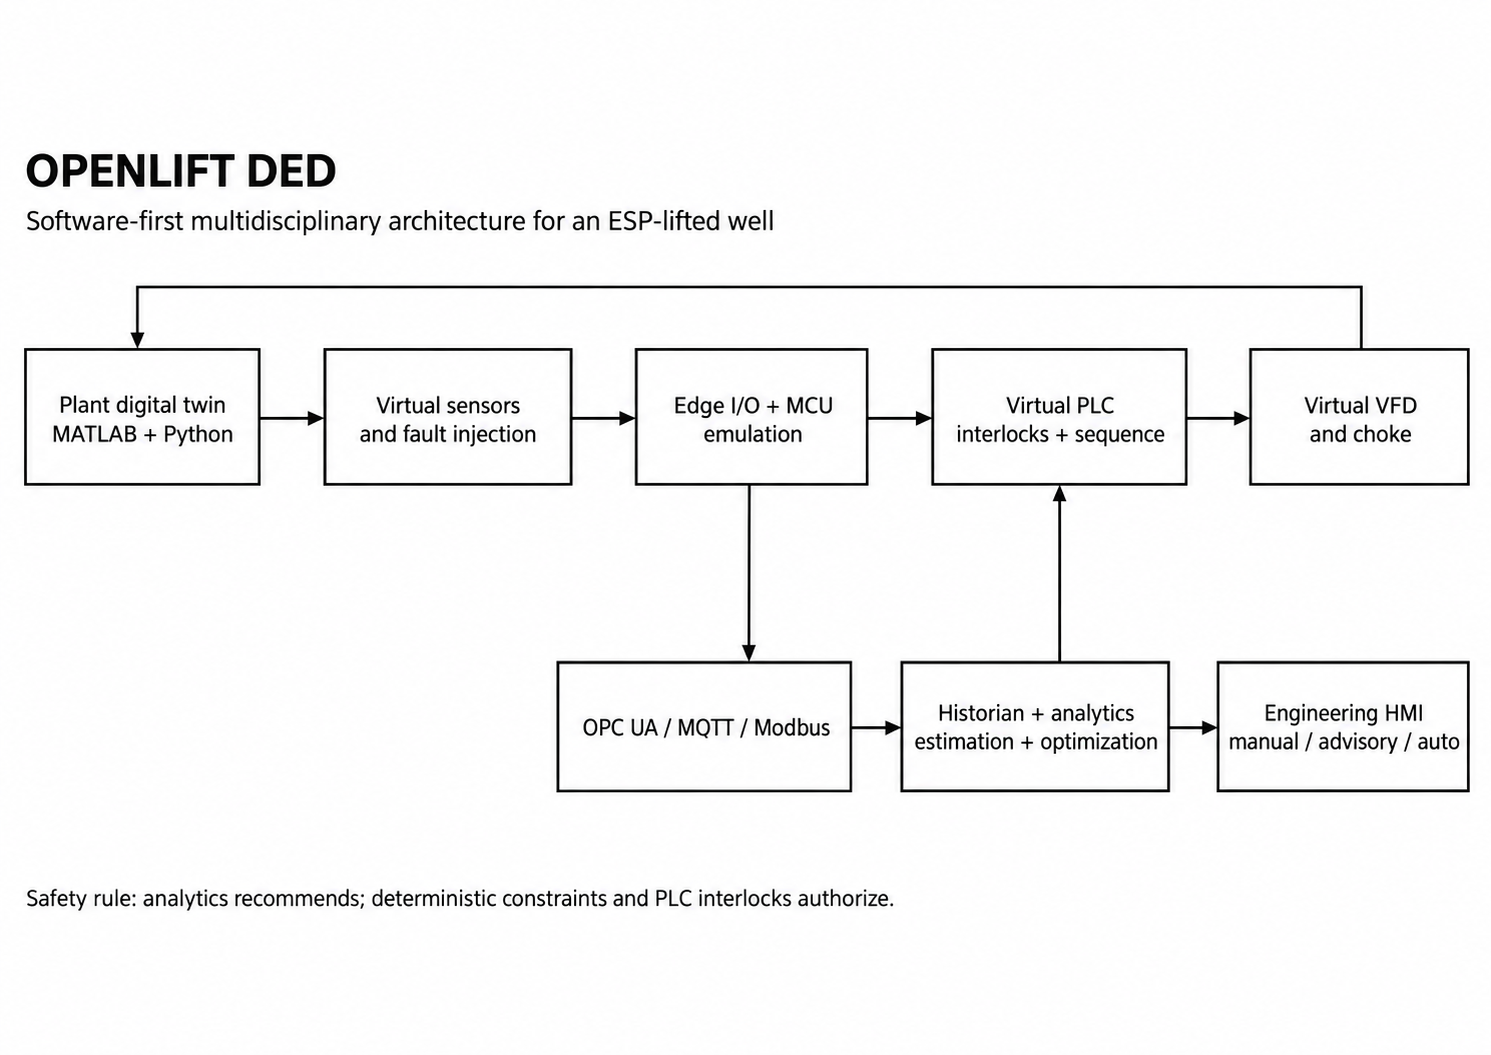
\includegraphics[width=0.96\textwidth]{system-architecture.png}
\caption{OpenLift DED reference architecture. The upper path represents deterministic plant-control execution. The lower path provides communication, history, analytics, and operator interaction. Analytical output cannot bypass PLC constraints and interlocks.}
\label{fig:architecture}
\end{figure*}

The virtual PLC is programmed using IEC 61131-3 concepts. IEC 61131-3 defines a unified suite of PLC programming languages and structures, while OpenPLC provides an accessible software implementation suitable for laboratory and research use \cite{iec61131,openplc}. FUXA is a candidate HMI/SCADA layer because its public documentation supports Modbus, OPC UA, and MQTT connectivity and a built-in historian path \cite{fuxa}. Tool selection remains replaceable; the interfaces and acceptance criteria are the durable design objects.

\subsection{Control Authority and Safety Precedence}
A research optimizer must not be treated as a safety instrumented function. OpenLift DED therefore separates command recommendation from deterministic authorization. The authority hierarchy is shown in Table~\ref{tab:authority}.

\begin{table}[t]
\caption{Control Authority Hierarchy}
\label{tab:authority}
\centering
\footnotesize
\begin{tabularx}{\columnwidth}{p{0.18\columnwidth}Y}
\toprule
Priority & Function \\
\midrule
1 & Hard trip and protective interlock \\
2 & Permissive and equipment operating envelope \\
3 & Degraded-mode and communications fallback \\
4 & Manual operator command within authorized limits \\
5 & Automatic PID/MPC command within authorized limits \\
6 & Analytics/health recommendation or derating request \\
\bottomrule
\end{tabularx}
\end{table}

The design follows defense-in-depth principles rather than claiming functional-safety compliance. IEC 62443-3-3 formalizes foundational security requirements for industrial automation and control systems, including identification/authentication, use control, system integrity, restricted data flow, timely response, and resource availability \cite{iec62443}. OpenLift DED uses those concepts as a design checklist for the laboratory architecture, but a software prototype is not an IEC 62443 certified system.

\section{Plant and Instrument Model}
\subsection{Reservoir Inflow}
The first reference model uses a linear productivity-index relation,
\begin{equation}
q_r = J\max(P_r-P_i,0),
\label{eq:ipr}
\end{equation}
where $q_r$ is reservoir inflow, $J$ is productivity index, $P_r$ is reservoir pressure, and $P_i$ is pump intake pressure. The model is intentionally replaceable by a nonlinear inflow relation after calibration. No claim is made that (\ref{eq:ipr}) captures multiphase inflow outside its declared validity envelope.

\subsection{Pump Head, Flow, and Power}
For a nominal speed $N_0$, a tabulated or fitted pump curve $H_0(q)$ is scaled using the centrifugal-pump affinity relation
\begin{equation}
H_p(q,N)=\left(\frac{N}{N_0}\right)^2
H_0\!\left(q\frac{N_0}{N}\right),
\label{eq:affinity}
\end{equation}
with analogous scaling for the reference flow axis. This is appropriate as a control-oriented approximation and must be bounded to the calibrated pump map \cite{takacs2018}. Pump differential pressure is
\begin{equation}
\Delta P_p = \rho g H_p,
\label{eq:headpressure}
\end{equation}
where $\rho$ is equivalent mixture density. Hydraulic and electrical power are
\begin{equation}
P_h=\rho g q H_p, \qquad
P_e=\frac{P_h}{\eta_p(q,N)\eta_m},
\label{eq:power}
\end{equation}
where $\eta_p$ and $\eta_m$ are pump and motor efficiencies. Efficiency is implemented as a bounded map rather than a constant when sufficient curve data are available.

\subsection{Lumped Pressure Dynamics}
Two compliance states provide a transparent transient model:
\begin{align}
C_i\dot P_i &= q_r-q_p, \label{eq:pi_dyn}\\
C_t\dot P_{wh} &= q_p-q_c, \label{eq:pwh_dyn}
\end{align}
where $q_p$ is pump/wellbore flow, $q_c$ is choke outflow, $P_{wh}$ is wellhead pressure, and $C_i,C_t$ are effective fluid/wellbore compliance terms. These states should be interpreted as control-oriented lumped storage, not as a detailed compressibility solution.

The choke model is
\begin{equation}
q_c=C_v(z_c)\sqrt{\frac{\max(P_{wh}-P_{sep},0)}{\rho}},
\label{eq:choke}
\end{equation}
where $z_c\in[0,1]$ is normalized choke position and $P_{sep}$ is downstream separator pressure. $C_v(z_c)$ is monotone and calibrated from a chosen valve characteristic.

\subsection{Actuator and Thermal Dynamics}
The VFD command is rate- and range-limited,
\begin{equation}
\tau_N\dot N=\sat(N_{cmd};N_{min},N_{max})-N,
\label{eq:vfd}
\end{equation}
with an independent ramp-rate limiter. A low-order motor thermal model is
\begin{equation}
C_{th}\dot T_m=P_{loss}-\frac{T_m-T_a}{R_{th}},
\label{eq:thermal}
\end{equation}
where $T_m$ is motor temperature and $P_{loss}$ is derived from electrical loading and efficiency. The model is suitable for testing thermal constraint handling, not for predicting absolute downhole temperature without calibration.

\subsection{Virtual Instrumentation and Fault Injection}
Each virtual measurement uses a configurable transfer function, sampling period, quantization, timestamp, noise distribution, and fault state. A generic measured signal is
\begin{equation}
y_m(t)=\mathcal{S}\{G_s(s)y(t)\}+b(t)+n(t),
\label{eq:sensor}
\end{equation}
where $G_s(s)$ is sensor dynamics, $\mathcal{S}$ denotes sample/hold and quantization, $b(t)$ is injected bias or drift, and $n(t)$ is noise. Fault modes include bias, ramp drift, freeze, dropout, stuck-at value, range clipping, packet delay, packet loss, timestamp skew, and implausible rate-of-change. Every injected fault carries a ground-truth label and activation interval.

\section{Control and State Estimation}
\subsection{Baseline Controllers}
Three control modes are compared under identical scenarios. The fixed-frequency baseline holds VFD speed at a prescribed setpoint and allows only protective overrides. The PID baseline regulates either intake pressure or production proxy with anti-windup, output saturation, ramp limiting, and bumpless mode transfer. The constrained controller uses a low-order state-space model and optimizes pump speed and, when enabled, choke position.

\subsection{State Estimation and Virtual Flow Meter}
An extended Kalman filter (EKF) and an unscented Kalman filter (UKF) are evaluated as interchangeable estimators. The state vector may include $P_i$, $P_{wh}$, $q$, an efficiency factor, and selected slowly varying disturbance states. The estimator outputs both state estimates and uncertainty. A virtual-flow estimate is never treated as equivalent to a calibrated custody or production meter; it is a control and surveillance variable whose error must be reported against the simulated ground truth or independent test-rig data.

A physics residual is defined by
\begin{equation}
r_k=y_k-\hat y^{\mathrm{phys}}_k,
\label{eq:residual}
\end{equation}
where $\hat y^{\mathrm{phys}}_k$ is generated by the estimator/model using the information available at time $k$. Residual construction must not leak future labels or test-set information.

\subsection{Constrained Model Predictive Control}
For manipulated variables $u=[N,z_c]^T$, the reference MPC minimizes
\begin{equation}
\begin{split}
J_c=\sum_{j=0}^{N_p} & w_p(P_{i,j}-P_{i,sp})^2
+w_q(q_j-q_{sp})^2 \\
&+w_E\,\tilde P_{e,j}+w_u\|\Delta u_j\|_2^2
+w_s\|\epsilon_j\|_2^2,
\end{split}
\label{eq:mpc}
\end{equation}
where $\tilde P_e$ is normalized electrical power and $\epsilon$ contains only explicitly soft constraints. Hard constraints include
\begin{align}
N_{min} &\le N_k\le N_{max}, \\
|\Delta N_k| &\le r_N, \\
P_i^{min} &\le P_{i,k}\le P_i^{max}, \\
I_{m,k} &\le I_m^{max}, \qquad T_{m,k}\le T_m^{max}, \\
z_c^{min} &\le z_{c,k}\le z_c^{max}.
\end{align}
The admissible envelope also includes a pump-flow region derived from the selected pump map. MPC is a natural fit because the ESP problem contains interacting variables and explicit constraints, consistent with prior ESP control studies \cite{pavlov2014,binder2014,krishnamoorthy2016}.

\subsection{Health-Aware Supervisory Derating}
The health model cannot directly bypass hard limits or interlocks. Instead, a calibrated risk score $h_k\in[0,1]$ can request a conservative upper operating bound,
\begin{equation}
N_{max,h}=N_{max}-\alpha_h\,g(h_k,\sigma_{h,k}),
\label{eq:derate}
\end{equation}
where $\sigma_{h,k}$ represents uncertainty and $g(\cdot)$ is monotone. If model confidence is low or an out-of-distribution condition is detected, authority is reduced rather than increased. This implements an uncertainty-aware fallback principle without presenting the health model as a safety function.

\section{Health Analytics and Data Design}
\subsection{Public Data Sources}
ESPset provides a real-world vibration dataset for ESP fault diagnosis and an experimental framework designed to reduce similarity bias between training and test samples \cite{varejao2024}. The paper reports 6032 vibration-test instances and shows that naive cross-validation can overestimate performance when dependent samples are split across folds. OpenLift DED therefore adopts grouped splitting for any ESPset experiment.

The 3W Dataset provides multivariate well-event data. Version 1 established a benchmark containing real, simulated, and hand-drawn instances \cite{vargas2019}; version 2.0.0 extends the public resource and retains explicit source categories and expert validation \cite{vargas2026}. Because these events arise from offshore well operations rather than the exact OpenLift asset, 3W performance is reported as external-dataset evidence, not direct validation of the proposed ESP controller.

\subsection{Learning Tasks}
Three analytics tasks are separated: (1) equipment condition classification from vibration features, (2) well-event detection from process time series, and (3) residual-based anomaly scoring from OpenLift scenarios. A single model is not forced to solve all tasks. Candidate baselines include logistic regression, random forest/gradient boosting, one-class methods, and temporal models where the data volume justifies them.

The minimum evaluation set includes macro-F1, class-wise precision and recall, precision-recall area, false alarms per operating day, detection lead time, expected calibration error, and performance across fault severity. The test protocol reports grouped and out-of-envelope results separately. Any hyperparameter selection is performed without access to the final test groups.

\section{Industrial Automation and Communications}
\subsection{PLC Responsibilities}
The PLC owns deterministic permissives, mode arbitration, start/stop sequence, interlocks, trip logic, first-out capture, command validation, watchdogs, and fallback. The preferred implementation language is Structured Text for state machines and reusable function blocks, with Ladder Diagram available for interlocks where visual review is beneficial. IEC 61131-3 provides the language framework \cite{iec61131}. OpenPLC is used as a research runtime because it supports IEC 61131-3 programming and virtual PLC execution \cite{openplc}.

A representative start permissive is
\begin{equation}
\begin{aligned}
Permissive ={}& HealthyIO \land CommOK \land \neg TripLatched \\
& \land LevelOK \land VFDReady.
\end{aligned}
\end{equation}
and no automatic command is accepted unless the requested mode, freshness, sequence state, and bounds are all valid. Trip reset requires the initiating condition to clear and an explicit reset action.

\subsection{Protocol Roles}
OPC UA is the preferred typed interface between supervisory applications because the standard defines a platform-independent information model, services, subscriptions, and security concepts for industrial interoperability \cite{opcua}. MQTT is reserved for decoupled event or telemetry publication where brokered publish/subscribe behavior is useful; MQTT 5.0 is standardized by OASIS \cite{mqtt5}. Modbus/TCP is retained for laboratory device emulation and compatibility because its request/reply application protocol remains widely implemented \cite{modbus}. It is not used as a justification for flat or unauthenticated production networking.

A practical tag model uses source timestamp, server timestamp, engineering unit, quality/status, validity, sequence number, and command freshness. A write command includes requested value, origin, mode, monotonic identifier, validity time, and acknowledgement. Stale commands are rejected.

\subsection{Cybersecurity Design Rules}
The laboratory architecture is segmented into control, supervisory, and analytics zones. Direct Internet exposure of the PLC or simulated field I/O is prohibited. OPC UA security modes and certificates are enabled when available; MQTT uses authenticated and encrypted transport in nonlocal deployments; Modbus is constrained to an isolated laboratory segment or a gateway boundary. Default credentials, anonymous remote write, shared administrator accounts, and permanent engineering write access are disallowed. Logs preserve command origin and configuration changes.

These controls are design measures only. Conformance to IEC 62443 requires a broader lifecycle, risk assessment, component capability, organizational process, and verification scope than this study provides \cite{iec62443}.

\section{HMI, Historian, and Operator Modes}
The HMI is an engineering interface rather than a decorative dashboard. It must show mode, command source, permissives, active trip, first-out event, VFD speed, choke position, intake and wellhead pressure, current proxy, motor temperature, flow estimate, estimator confidence, communication status, health score, and constraint margin. Alarm design distinguishes process alarm, equipment trip, instrumentation fault, communications fault, and analytics advisory.

Supported modes are \emph{Manual}, \emph{Advisory}, \emph{Automatic}, \emph{Degraded}, \emph{Trip}, \emph{Fault Injection}, and \emph{Replay}. Fault Injection is available only in simulation and is visually unmistakable. Replay cannot write to the live controller namespace. FUXA is a candidate open HMI because it supports web-based process visualization, common industrial protocols, and data history \cite{fuxa}.

The historian stores raw measurements, validated measurements, estimated states, commands, command source, controller status, model version, scenario identifier, injected-fault labels, alarms, and timing metadata. Configuration changes are versioned separately from measurements.

\section{Virtual Commissioning Protocol}
\subsection{Verification Stages}
The commissioning process is staged so that evidence maturity is clear.

\textbf{Stage 0: Static engineering review.} Requirements, tag register, I/O mapping, units, ranges, alarm list, cause-and-effect, state-machine transitions, network endpoints, and diagram consistency are reviewed before dynamic tests.

\textbf{Stage 1: Model-in-the-loop (MIL).} Plant equations and controller execute in one numerical environment. Unit models are checked for conservation, monotonicity, limiting behavior, sign convention, and sensitivity.

\textbf{Stage 2: Software-in-the-loop (SIL).} Controller, estimator, historian, and analytics execute as independent software modules connected through the defined interfaces. Serialization, sampling, timestamps, and data-quality rules become part of the test.

\textbf{Stage 3: Controller-in-the-loop (CIL).} The plant simulator and software PLC execute as separate processes. The PLC scan, I/O update, protocol timing, command freshness, watchdogs, fallback, and first-out behavior are measured.

\textbf{Stage 4: Hardware-in-the-loop (HIL).} Deferred. Physical controller or I/O hardware is required before this term is used. The initial project must not label software-only tests as HIL.

\subsection{Scenario Matrix}
Table~\ref{tab:scenarios} defines the minimum reference campaign. Severity, onset shape, duration, and random seed are parameterized so the same scenario can be replayed across controllers.

\begin{table*}[t]
\caption{Minimum Virtual Commissioning Scenario Matrix}
\label{tab:scenarios}
\centering
\footnotesize
\begin{tabularx}{\textwidth}{p{0.08\textwidth}p{0.20\textwidth}Y Y p{0.17\textwidth}}
\toprule
ID & Scenario & Injection & Expected safe behavior & Principal evidence \\
\midrule
S0 & Nominal production & No fault; setpoint changes & Track within envelope & Tracking, energy, latency \\
S1 & Reservoir depletion & Ramp $P_r$ or reduce $J$ & Re-optimize without violating $P_i$ floor & Constraint margin, production \\
S2 & Hydraulic restriction & Increase tubing/choke loss & Detect residual; avoid over-speed & Residual, current/thermal margin \\
S3 & Gas-interference surrogate & Reduce head/efficiency factor & Derate or stabilize; no repeated trip cycling & Speed, $P_i$, thermal state \\
S4 & Pump efficiency loss & Gradual $\eta_p$ reduction & Increased energy detected; advisory health flag & kWh/m$^3$, residual trend \\
S5 & Pressure-sensor bias & Step/ramp bias & Innovation/quality alarm; estimator uncertainty rises & Estimator error, detection delay \\
S6 & Sensor dropout/freeze & Missing/stale value & Timeout; bounded fallback or degraded mode & Mode transition, constraint compliance \\
S7 & Network delay/loss & Delay, jitter, packet loss & Reject stale writes; preserve safe local control & Deadline, stale-command rejection \\
S8 & Bad optimizer command & Out-of-range or contradictory command & PLC rejects/clamps according to policy & 100\% unsafe-command containment \\
S9 & VFD/choke actuator fault & Stuck/rate-limited actuator & Detect tracking mismatch; safe fallback/trip if needed & Residual, first-out, recovery \\
S10 & Model mismatch & Perturb density, friction, efficiency & Maintain robustness or expose limitation & Error by mismatch magnitude \\
S11 & OOD operating point & Outside training envelope & Lower analytics authority; raise OOD status & OOD recall, safe mode \\
\bottomrule
\end{tabularx}
\end{table*}

\section{Evaluation Metrics and Acceptance Criteria}
Control performance is reported using normalized RMSE, integrated absolute error (IAE), overshoot, settling time, produced volume, electrical energy, energy intensity, minimum constraint margin, control effort, and mode transitions. Timing reports scan time and solver latency using P50, P95, P99, maximum, and deadline-miss count. Safety evidence reports each injected hazardous request and its disposition.

Estimator performance uses RMSE, normalized innovation statistics where applicable, uncertainty coverage, dropout recovery time, and error conditioned on operating region. Analytics use grouped-test classification metrics, precision-recall area, false alarms per operating day, calibration, detection lead time, and performance versus fault severity.

Table~\ref{tab:criteria} lists initial project gates. These values are engineering targets to be revised after model calibration and baseline runs.

\begin{table*}[t]
\caption{Initial Acceptance Criteria for the Reference Campaign}
\label{tab:criteria}
\centering
\footnotesize
\begin{tabularx}{\textwidth}{p{0.25\textwidth}p{0.20\textwidth}Y p{0.19\textwidth}}
\toprule
Measure & Initial criterion & Interpretation & Evidence source \\
\midrule
Requirements traceability & 100\% of safety/control requirements mapped to a test & No orphan critical requirement & Traceability matrix \\
Critical PLC interlocks & 100\% pass & Every specified trip/permissive test behaves as designed & Automated CIL test log \\
Unsafe advisory commands & 100\% contained & No out-of-envelope analytics command reaches plant actuation & Fault campaign \\
Hard-constraint violations & Zero in reference campaign & Reference test suite must remain inside declared hard limits & Scenario logs \\
Normalized intake-pressure RMSE & $<5\%$ of declared operating span & State/control quality target, not field accuracy claim & Held-out scenarios \\
Steady production tracking error & $<5\%$ after settling in nominal cases & Baseline target for matched comparison & S0/S1 \\
Energy-intensity improvement & $>5\%$ in at least one predeclared variable-load scenario & Must not be obtained by violating constraints or reducing required production & Matched controller comparison \\
MPC deadline misses & 0; P99 below control interval & Real-time feasibility within defined software/hardware setup & Timing log \\
Sensor failure handling & Degraded or safe state within configured timeout & No silent use of indefinitely stale critical data & S5/S6 \\
OOD handling & Authority not increased under OOD flag & Uncertainty must be fail-conservative & S11 \\
Reproducibility & One-command reference campaign from tagged release & Environment, seed, configuration, and results are versioned & Clean-machine reproduction \\
\bottomrule
\end{tabularx}
\end{table*}

\subsection{Statistical Analysis}
Controller comparisons use identical scenario parameter sets and random seeds. Results are aggregated across a predeclared set of operating points and fault severities. Mean or median alone is insufficient; distributions and confidence intervals are reported. When the number of scenario replicates is modest, bootstrap confidence intervals are preferred over unsupported normality assumptions. For analytics, the grouping unit is defined before training, and the final test groups are not used for threshold tuning.

Ablations compare (1) raw sensors versus physics residuals versus combined features, (2) PID versus MPC, (3) MPC versus health-aware bounded MPC, (4) estimator with and without adaptive disturbance states, and (5) nominal communications versus delay/loss. Negative results remain part of the study.

\section{Reproducibility and Engineering Traceability}
The repository is organized so that configuration, implementation, and generated evidence cannot be confused. A proposed structure is:
\begin{table}[h]
\caption{Proposed Repository Layout}
\label{tab:repo}
\centering
\scriptsize
\begin{tabularx}{\columnwidth}{p{0.26\columnwidth}Y}
\toprule
Folder & Purpose \\
\midrule
\texttt{requirements/} & Requirements and traceability \\
\texttt{process/} & Equations, parameters, PFD/P\&ID \\
\texttt{plc/} & IEC 61131-3 source and tests \\
\texttt{edge/} & I/O emulator and protocol maps \\
\texttt{control/} & PID, estimator, and MPC \\
\texttt{analytics/} & Datasets, features, models, cards \\
\texttt{hmi/} & Screens, alarms, navigation \\
\texttt{electrical/} & Conceptual power/control package \\
\texttt{pcb/} & Interface-board design artifacts \\
\texttt{mechanical/} & CAD concepts and interfaces \\
\texttt{scenarios/} & Versioned scenario definitions \\
\texttt{tests/} & MIL/SIL/CIL automated tests \\
\texttt{evidence/} & Generated logs, figures, reports \\
\texttt{docs/} & Basis of design and study report \\
\bottomrule
\end{tabularx}
\end{table}

Each requirement receives a stable identifier, verification method, test identifier, and pass/fail evidence location. Each experiment records code commit, configuration hash, model version, scenario identifier, seed, environment, controller version, and timestamp. Public dataset experiments also record dataset release and split manifest.

The automation interface follows open industrial standards where practical. OPC UA provides the main typed supervisory interface \cite{opcua}; MQTT 5.0 provides an optional event/telemetry transport \cite{mqtt5}; Modbus/TCP provides constrained compatibility testing \cite{modbus}. These protocols are implementation options, not a requirement that all three operate simultaneously in every test.

\section{Engineering Work Packages}
The project is multidisciplinary, but the deliverables are bounded by evidence level.

\subsection{Process and Instrumentation}
Deliverables include basis of design, process flow diagram, simplified P\&ID, tag register, instrument index, I/O list, alarm list, cause-and-effect matrix, control narrative, model derivation, validity envelope, and parameter source register.

\subsection{Electrical and Embedded Interfaces}
The electrical package defines conceptual VFD/motor supply, auxiliary 24-VDC control supply, protective-device assumptions, terminal plan, cable schedule, grounding concept, and I/O segregation. The embedded package defines a virtual or later physical sensor interface for 4--20 mA, 0--10 V, 24-V digital I/O, isolated RS-485, watchdog, and diagnostics. No hazardous-area suitability, insulation coordination, EMC compliance, or certified protection claim is made without dedicated design and test evidence.

\subsection{Mechanical and PCB Digital Design}
Mechanical CAD and PCB artifacts exist to preserve interfaces and test engineering consistency. CAD checks include mounting envelope, connector access, collision, service clearance, and revision control. PCB checks include electrical-rule check, design-rule check, protection topology review, isolation boundary review, connector pinout consistency, and bill of materials. These are design-review artifacts, not manufactured-equipment qualification.

\section{Risks, Failure Modes, and Validity Limits}
The largest technical risk is \emph{model credibility}. A low-order simulator can reward a controller for exploiting assumptions that do not survive real multiphase behavior. The mitigation is to declare the validity envelope, perturb parameters, compare against literature behavior, and avoid claiming field performance.

The second risk is \emph{data leakage}. ESPset explicitly demonstrates that dependent sampling can inflate apparent machine-learning performance \cite{varejao2024}. Group manifests and immutable held-out test groups are therefore mandatory.

The third risk is \emph{authority creep}, where a useful analytics prototype gradually becomes able to issue unbounded control actions. The mitigation is a fixed PLC authorization boundary, command freshness checks, mode arbitration, and test cases that deliberately send unsafe commands.

The fourth risk is \emph{timing blindness}. A numerically optimal controller that misses deadlines is not operationally equivalent to a deterministic controller. Execution-time distributions are therefore first-class results.

The fifth risk is \emph{cybersecurity overclaim}. Using OPC UA certificates or network segmentation does not establish IEC 62443 compliance. The study uses selected requirements as design guidance only \cite{iec62443}.

The initial plant omits detailed PVT behavior, free-gas dynamics, multiphase flow correlations, pump-stage geometry, cable voltage drop and harmonics, motor electromagnetic dynamics, detailed shaft thrust, bearing dynamics, scale/corrosion chemistry, high-fidelity heat transfer, separator dynamics, facility constraints, and reservoir spatial dynamics. The model also does not prove hazardous-area, functional-safety, electrical-code, cybersecurity, or environmental compliance. These exclusions define the boundary of valid conclusions.

\section{Implementation Plan}
Table~\ref{tab:plan} defines a part-time implementation sequence. A phase is complete only when its gate evidence is available.

\begin{table}[t]
\caption{Proposed Implementation Plan}
\label{tab:plan}
\centering
\footnotesize
\begin{tabularx}{\columnwidth}{p{0.10\columnwidth}Y p{0.16\columnwidth}}
\toprule
Phase & Gate output & Duration \\
\midrule
0 & Requirements, literature register, tags, criteria & 2 wk \\
1 & Plant model, parameter set, open-loop verification & 4 wk \\
2 & PID, EKF/UKF, MPC, timing harness & 4 wk \\
3 & PLC, edge I/O, protocols, historian, HMI & 4 wk \\
4 & Electrical, PCB, mechanical digital package & 4 wk \\
5 & Health analytics and grouped dataset evaluation & 5 wk \\
6 & SIL/CIL fault campaign and ablations & 4 wk \\
7 & Report, release, video, archive, reproducibility test & 3 wk \\
\bottomrule
\end{tabularx}
\end{table}

The minimum public release contains source code, environment lock file, requirements and traceability matrix, scenario definitions, controller configurations, dataset split manifests, model and dataset cards, automated tests, generated reference figures, a virtual FAT report, known limitations, and a software bill of materials. A DOI is added only after a reviewed release is archived.

\section{Expected Outcomes}
A successful study will not be defined by the highest production number or machine-learning score. It will be defined by whether the project can show, with reproducible evidence, how performance changes when constraints, timing, data quality, uncertainty, and failure modes are introduced. The principal expected outcome is an engineering reference system in which the same scenario can be replayed across fixed-speed, PID, and MPC control while preserving identical plant conditions and fault injections.

A second expected outcome is a clear separation between analytical recommendation and deterministic authorization. This permits health-aware optimization experiments without representing a statistical model as a protective layer. A third outcome is a reusable multidisciplinary interface: the same tag and requirement definitions drive the process model, PLC, HMI, communications, electrical concept, PCB interface, and validation report.

\section{Conclusion}
OpenLift DED defines a reproducible path from ESP process physics to virtual commissioning while keeping evidence level and control authority explicit. Prior ESP research supports model-based constrained control, and public datasets support realistic condition-monitoring experiments, but a credible engineering study must also account for sensor validity, communications, deterministic protection, timing, operator modes, and traceability. The proposed architecture addresses those elements as a single system. Its central safety rule is simple: analytics can advise and optimize within a bounded envelope, while PLC constraints and interlocks authorize actuation. The initial release remains a software-first research platform; HIL, field calibration, certification, and production deployment require separate evidence. Within that boundary, the study can produce a technically defensible open baseline for multidisciplinary ESP automation research.

\begin{thebibliography}{99}

\bibitem{takacs2018}
G. Takacs, \emph{Electrical Submersible Pumps Manual: Design, Operations, and Maintenance}, 2nd ed. Gulf Professional Publishing, 2018, doi: 10.1016/C2017-0-01308-3.

\bibitem{pavlov2014}
A. Pavlov, D. Krishnamoorthy, K. Fjalestad, E. Aske, and M. Fredriksen, ``Modelling and model predictive control of oil wells with Electric Submersible Pumps,'' in \emph{Proc. 2014 IEEE Conf. Control Applications (CCA)}, 2014, pp. 586--592, doi: 10.1109/CCA.2014.6981403.

\bibitem{binder2014}
B. J. T. Binder, D. K. M. Kufoalor, A. Pavlov, and T. A. Johansen, ``Embedded Model Predictive Control for an Electric Submersible Pump on a Programmable Logic Controller,'' in \emph{Proc. 2014 IEEE Conf. Control Applications (CCA)}, 2014, pp. 579--585, doi: 10.1109/CCA.2014.6981402.

\bibitem{krishnamoorthy2016}
D. Krishnamoorthy, E. M. Bergheim, A. Pavlov, M. Fredriksen, and K. Fjalestad, ``Modelling and robustness analysis of model predictive control for electrical submersible pump lifted heavy oil wells,'' \emph{IFAC-PapersOnLine}, vol. 49, no. 7, pp. 544--549, 2016, doi: 10.1016/j.ifacol.2016.07.399.

\bibitem{erickson2024}
R. Erickson, R. Ramos, J. Meek, D. Benham, B. Haapanen, B. Hicks, C. Wheeler, and B. Vasylyshyn, ``Autonomous ESP Optimization Using Machine Learning Demonstrated in the Permian Basin,'' in \emph{SPE Artificial Lift Conference and Exhibition - Americas}, 2024, Paper SPE-219528-MS, doi: 10.2118/219528-MS.

\bibitem{varejao2024}
F. M. Varejao, L. H. S. Mello, M. P. Ribeiro, T. Oliveira-Santos, and A. L. Rodrigues, ``An open source experimental framework and public dataset for vibration-based fault diagnosis of electrical submersible pumps used on offshore oil exploration,'' \emph{Knowledge-Based Systems}, vol. 288, Art. no. 111452, 2024, doi: 10.1016/j.knosys.2024.111452.

\bibitem{vargas2019}
R. E. V. Vargas, C. J. Munaro, P. M. Ciarelli, A. G. Medeiros, B. G. Amaral, D. C. Barrionuevo, J. C. D. Araujo, J. L. Ribeiro, and L. A. P. Magalhaes, ``A realistic and public dataset with rare undesirable real events in oil wells,'' \emph{Journal of Petroleum Science and Engineering}, vol. 181, Art. no. 106223, 2019, doi: 10.1016/j.petrol.2019.106223.

\bibitem{vargas2026}
R. E. V. Vargas \emph{et al.}, ``3W Dataset 2.0.0: a realistic and public dataset with rare undesirable real events in oil wells,'' \emph{Scientific Data}, vol. 13, Art. no. 949, 2026, doi: 10.1038/s41597-026-07225-z.

\bibitem{slb-intelligent}
SLB, ``Intelligent Lift,'' accessed Sep. 11, 2026. [Online]. Available: \url{https://www.slb.com/products-and-services/innovating-in-oil-and-gas/completions/artificial-lift/intelligent-lift}

\bibitem{slb-loa}
SLB, ``Lift operations advisor,'' accessed Sep. 11, 2026. [Online]. Available: \url{https://www.slb.com/products-and-services/delivering-digital-at-scale/production/production-operations/lift-operations-advisor}

\bibitem{slb-liftiq}
SLB, ``Lift IQ production life cycle management service,'' accessed Sep. 11, 2026. [Online]. Available: \url{https://www.slb.com/products-and-services/innovating-in-oil-and-gas/completions/artificial-lift/optimizing-artificial-lift/lift-iq-production-life-cycle-management-service}

\bibitem{iec61131}
PLCopen, ``IEC 61131-3,'' programming languages for programmable controllers, accessed Sep. 11, 2026. [Online]. Available: \url{https://www.plcopen.org/standards/logic/iec-61131-3/}

\bibitem{opcua}
OPC Foundation, ``OPC Unified Architecture - Part 1: Overview and Concepts,'' OPC 10000-1, accessed Sep. 11, 2026. [Online]. Available: \url{https://reference.opcfoundation.org/specs/OPC-10000-1/}

\bibitem{mqtt5}
A. Banks, E. Briggs, K. Borgendale, and R. Gupta, eds., ``MQTT Version 5.0,'' OASIS Standard, Mar. 7, 2019. [Online]. Available: \url{https://docs.oasis-open.org/mqtt/mqtt/v5.0/mqtt-v5.0.html}

\bibitem{modbus}
Modbus Organization, ``MODBUS Application Protocol Specification V1.1b3,'' 2012. [Online]. Available: \url{https://www.modbus.org/docs/Modbus_Application_Protocol_V1_1b3.pdf}

\bibitem{iec62443}
IEC, \emph{IEC 62443-3-3:2013, Industrial Communication Networks - Network and System Security - Part 3-3: System Security Requirements and Security Levels}. Geneva, Switzerland: International Electrotechnical Commission, 2013.

\bibitem{openplc}
Autonomy, ``OpenPLC Runtime v4,'' accessed Sep. 11, 2026. [Online]. Available: \url{https://autonomylogic.com/runtime}

\bibitem{fuxa}
FrangoTeam, ``FUXA: Web-based Process Visualization (SCADA/HMI/Dashboard) software,'' accessed Sep. 11, 2026. [Online]. Available: \url{https://github.com/frangoteam/FUXA}

\end{thebibliography}

\end{document}
